\section{Planification}

\subsection{Planification des fonctionnalités}

Notre robot permet d'aider un individu ayant les faculté affaibli à jouer au bière-pong.
On intéragi avec lui via une application Android.

Au début du projet, nous avons identifié plusieurs fonctionnalité d'un produit final.
La liste qui suit les énumères.

\begin{enumerate}
    \item Lance avec précision
    \item Joue des chansons
    \item Danse/Célèbre la victoire de l’équipe du propriétaire
    \item Se déplace et lance automatiquement ou manuellement à l’aide d’une manette contrôlé par un humain
    \item Communique avec les verres pour savoir si le lancer est réussi ou non
    \item Écœure l’autre équipe (joue la chanson sad violon quand ils manquent les verres)
    \item Contrôlable pour viser les joueurs de l’autre équipe
\end{enumerate}

Nous avons jugé que certaines de ces fonctionalités n'étaient pas nécessaires pour un prototype.
À partir des fonctionalité restante, nous avons planifié de les concevoir et de les implémenter selon l'échéanchier du diagramme de Gantt de la figure~\ref{fig:planif-initial}.
À ce moment, nous avons décidé de conserver les dernières trois semaines afin de remplir des documents, d'effectuer des tests, d'absorber des retards, etc.

Au cours du projet, nous avons ajouté des tâches et nous avons pris la décision de retirer certaines tâches dont nous jugions moins pertinente.
Par exemple, nous avons imprimé des pièces avec n'importe quelle couleur.
Afin d'obtenir un robot avec des pièces d'une couleur uniforme, nous avons dû ajouter une tâche pour imprimer les pièces de la même couleur.

Vers la fin du projet, nous avons constaté que la planification initiale n'était plus réaliste.
En effet, plusieurs tâches n'avait pas encore été réalisés.
Nous avons donc planifier d'effectuer ces tâches dans les trois dernières semaines selon l'échéanchier du diagramme de Gantt de la figure~\ref{fig:planif-final}.

\begin{figure}[h!]
    \centering
    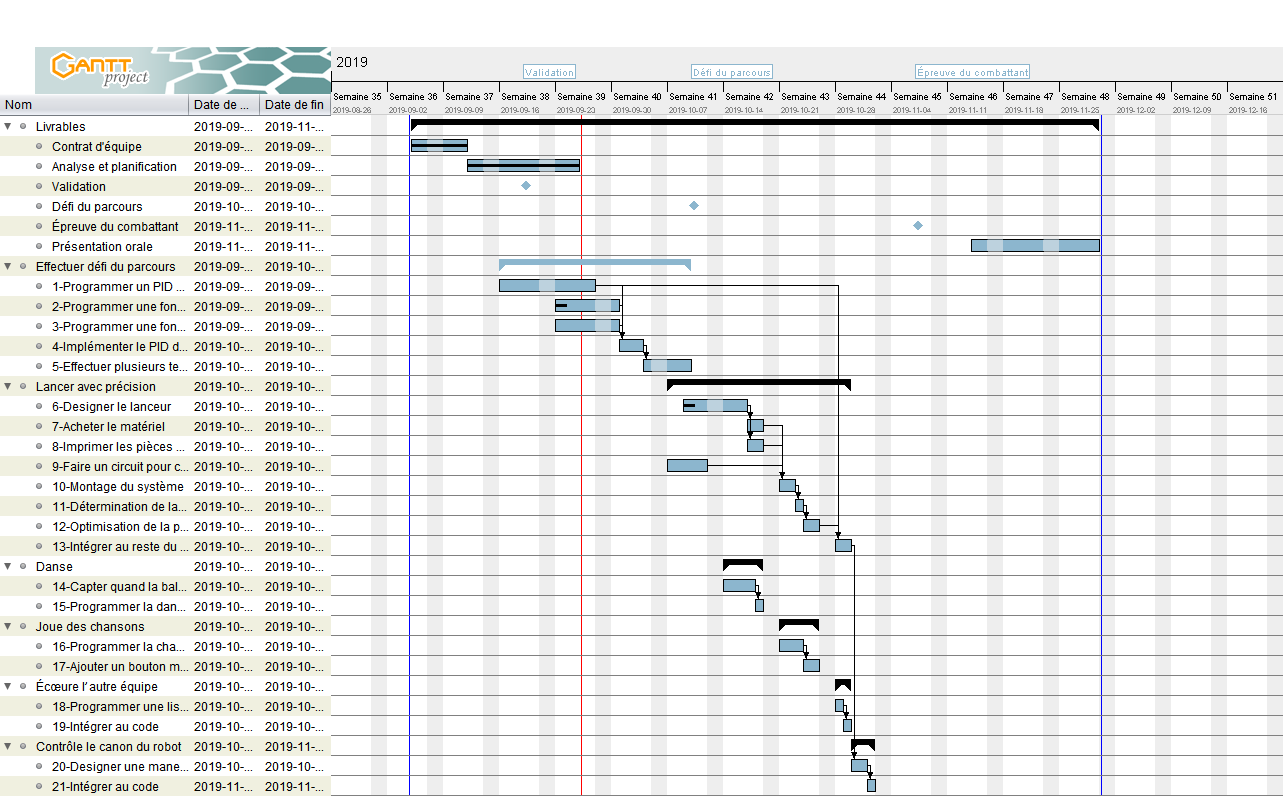
\includegraphics[width=\linewidth]{img/s1/robuck-2019-09-26}
    \caption{Diagramme de Gantt intial}
    \label{fig:planif-initial}
\end{figure}

\begin{figure}[h!]
    \centering
    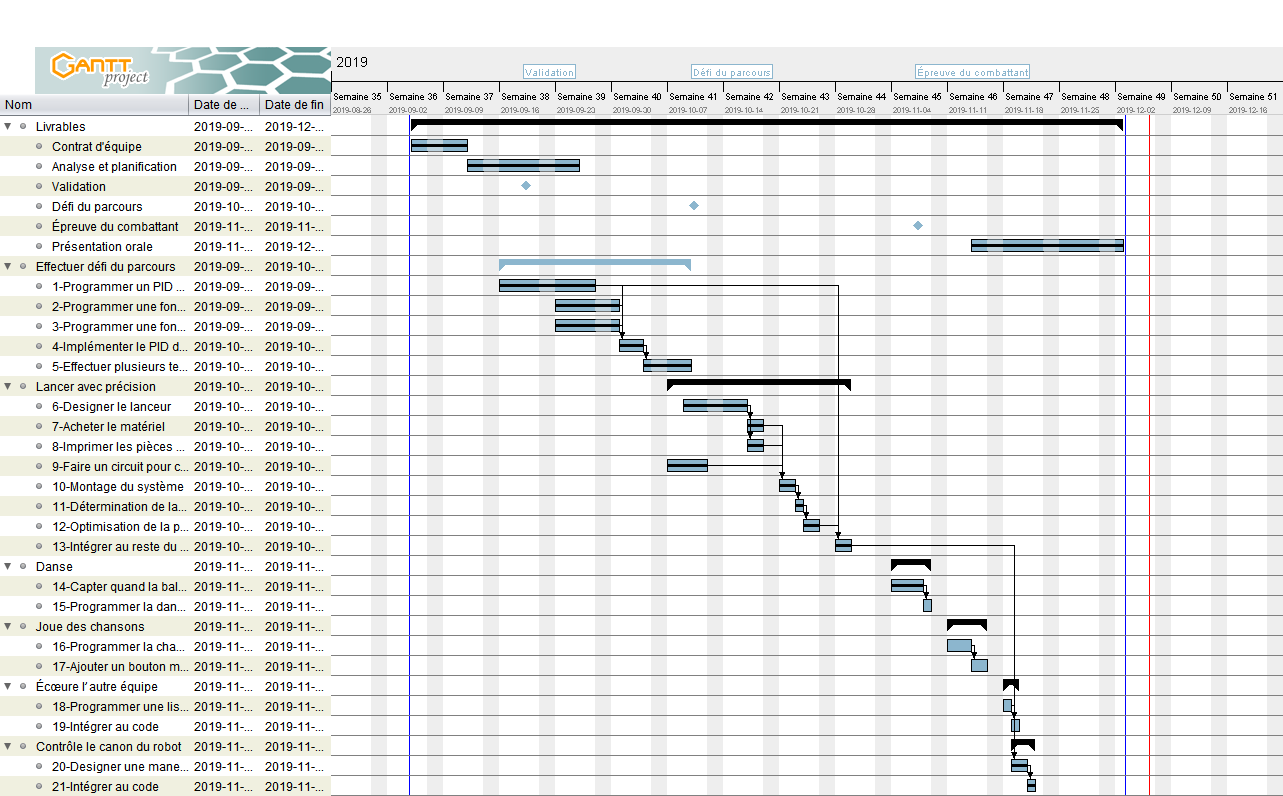
\includegraphics[width=\linewidth]{img/s1/robuck-2019-12-06.png}
    \caption{Diagramme de Gantt final}
    \label{fig:planif-final}
\end{figure}

\clearpage

\subsection{Gestion du projet et outils}

Nous avons tenu des réunions hebdomadaires de suivis.
Ces rencontres nous ont permis d'ajuster la distribution hebdomadaires des tâches.

Nous avons implémenté un tableau de bord de type Kanban à l'aide du service Trello tel qu'illustré à la figure~\ref{fig:planif-trello}.
Ce tableau nous a aider à prioriser les tâches lors des réunions hebdomadaire.

\begin{figure}[h!]
    \centering
    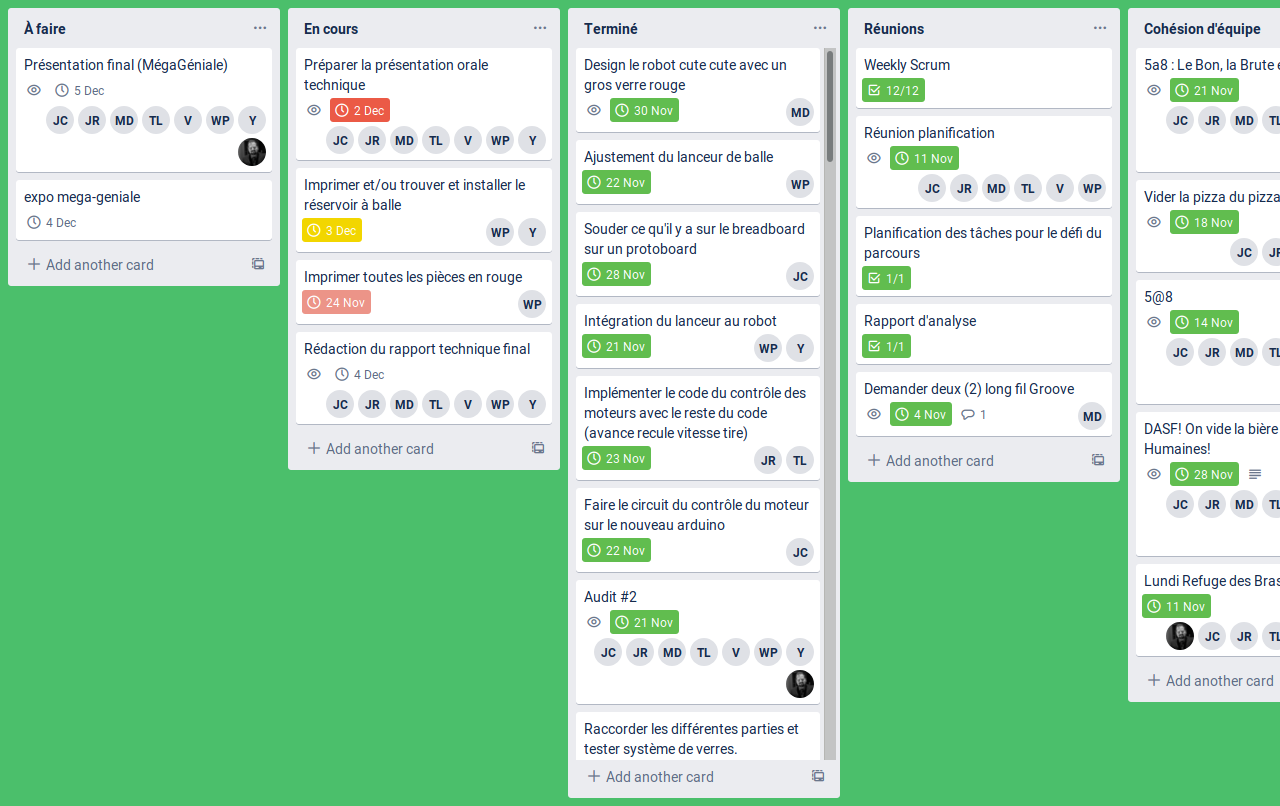
\includegraphics[width=\linewidth]{img/s1/trello}
    \caption{Implémentation d'un Kanban à l'aide de Trello}
    \label{fig:planif-trello}
\end{figure}

Nous avons utilisé plusieurs canaux de communications.
D'abord, lorsque c'était possible, nous communiquions de vive voix.
Lorsque ce n'était pas possible, nous utilisions le service Messenger de Facebook ou l'adresse courriel de l’Université de Sherbrooke.
Enfin, nous hébergions des fichiers avec le service d'hébergement de GitHub et sur un groupe SharePoint de Microsoft.
